\documentclass[10pt]{article}
\usepackage{verbatim}
\usepackage{multirow}
\usepackage{fullpage}
\usepackage{graphicx}
\usepackage{parskip}

\pagestyle{plain}

\title{{\normalsize CSCI 572: Computer Networks (Fall 2023)}\\Proposal: Ad-Hoc Messaging App}
\author{Michael Alvarez, Luke Beukelman, Ben Breisch}
\date{October 9th 2023}

\begin{document}

\maketitle

\section{Introduction}
% Motivate the problem;
% Define/formulate the problem: assumptions, application requirements, goals and non-goals;
If someone wants to send a message to a friend nearby, the message must travel much farther than the distance between devices. Messages sent through SMS or Apple's iMessage must travel from the originating device through a series of intermediate infrastructure nodes before reaching the destination device. This causes increased latency and unnecessary network overhead. In an increasingly connected (and congested) world - why bother wasting bandwidth on a message to a nearby device that can be sent directly from peer to peer? We aim to solve this issue by proposing and developing a peer-to-peer messaging app for Android using Wi-Fi Direct for multi-hop ad-hoc networking. An application of this nature has far-reaching applications from messaging and networking at an event or conference to emergency communication during a natural disaster. Although security is always an issue with wireless communication, that is out of the scope of this project. The table below shows some preliminary requirements for this proposed solution.
\begin{center}
    \begin{tabular}{| p{0.2\textwidth} | p{0.5\textwidth} |}
        \hline
        Category        & Requirement                                                                                                     \\ \hline
        Networking      & Connections between two devices shall use Wi-Fi Direct using the Android Wi-Fi P2P API                          \\ \hline
        Networking      & Devices shall provide routing of messages between source and destination nodes using a to-be-determined routing protocol. \\ \hline
        Networking      & Devices shall provide acknowledgements when messages are received in order to ensure message delivery           \\ \hline
        User Experience & Users shall be able to send text and file messages                                                              \\ \hline
        User Experience & Latency shall be minimized as much as possible when sending messages (ideally within 1 second)                  \\ \hline
        User Experience & Devices shall save messages offline such that they can be viewed later                                          \\ \hline
        User Experience & Devices shall show a contact list of other nearby users that a user can start a conversation with               \\ \hline
        User Experience & Devices shall show a contact list of other nearby users that a user can start a conversation with               \\ \hline
    \end{tabular}
\end{center}

\newpage

\section{Related work}
%\item What has been done before?
%\item How does your solution compare to them?

\subsection{AirDrop}

When it comes to ad hoc networking on mobile devices, AirDrop is probably the most widespread application. It supports sending files to nearby devices, without requiring devices to be connected to the same network. AirDrop operates using both Wi-Fi and Bluetooth \cite{AppleSupport}.

We aim to differ from this product in several regards:
\begin{enumerate}
    \item We primarily aim to support messaging. Having file sharing as a back end is a possible implementation to build messaging on, but would need to be extended.
    \item AirDrop uses iCloud services in order to authenticate users \cite{AppleSupportSecurity}, and additionally only works on Apple devices. We aim to create a de-centralized version that
          could theoretically be deployed on any platform (although we are only developing the application for Android in the scope of this project).
    \item AirDrop uses a combination of point-to-point WiFi connections and bluetooth. We aim to only use Ad-Hoc Wi-Fi / Wi-Fi Direct in our implementation. We realize that the technology choice restricts what devices we can connect with (Apple does not support Wi-Fi direct).
\end{enumerate}

\subsection{Warpinator}

Warpinator is a file sharing system devloped by the Linux Mint team in order to create an AirDrop like file-sharing system for non-Apple users  \cite{Webster2023linuxmint}. It operates over
LAN, and supports Android, iOS, Windows, and Linux, and could likely be easily ported to other Unix like systems.

We aim to differ from this product in two regards:
\begin{enumerate}
    \item As in AirDrop, we primarily aim to support messaging
    \item Operate using ad-hoc networking to support messaging. Warpinator requires a connection to an existing routed network, and can not operate its own ad-hoc network.
\end{enumerate}

\subsection{Android Beam}
Android beam is a discontinued \cite{Cantisano_2022} feature in Android that allowed data to be transfered over NFC \cite{AndroidDevelopers}. Unlike the prior two works, Android Beam did not only support file
transfer, and was an open interface that applications could use to communicate. Android Beam could provide a reasonable interface for a similar application as ours
to communicate with, if it were not discontinued and limited to NFC.

We aim to differ from this product in two regards:
\begin{enumerate}
    \item We aim to use WiFi technologies, rather than NFC, due to the short range limitation of NFC.
    \item We are creating an application, rather than an open interface to communicate over.
\end{enumerate}

\newpage

\subsection{A Totally Decentralized Document Sharing System for Mobile Ad Hoc Networks}
This paper  \cite{10.1145/1164783.1164805} presents an application for sharing documents in MANETS. The application presented
is completely unreliant on any form of centralized server or routing algorithms. Documents can be shared in atomic components to different groups
of nodes, and nodes can modify parts of a document, sharing a tree of the modifications. This application achieves a lot of what we are trying to
do, except with more routing and versioning complexity than we are seeking. Our goal is simple messaging and possible document sharing with nearby
nodes, not necessarily using MANET routing algorithms.

We aim to differ from this product in two regards:
\begin{enumerate}
    \item Our solution aims to target simple messaging and file sharing, rather than the complex sharing and versioning that the application in the paper presents.
    \item We don't intend to use novel or extremely complex routing algorithms such as those used in MANETS, our goal is short range communications within the range of phone antennas however it may be achieved.
\end{enumerate}

% There are some existing apps available for Android and iOS. Many of these apps use Bluetooth
% https://engage.sinch.com/blog/offline-messaging-apps/ \\
% https://apps.apple.com/us/app/walkie-talkie-p2p/id1181349764 \\
% https://ieeexplore.ieee.org/document/9473791 \\
% https://arxiv.org/abs/1601.00028 \\
% https://github.com/NaniteFactory/Wifi-Direct-on-Linux \\
% https://github.com/tigewilliams/WifiDirect

\section{Approach} %(optional)
%    \item Rationale: Why is it a good idea?
%     \item Sketch of your approach and design.
Mobile app development, especially for Android, has an extremely wide range of resources on the Internet. The Android platform is well supported by the community and we plan to leverage online resources for the development of this app. Android provides an existing Wi-Fi Direct library that we will leverage to speed up development. We will develop this app using Android's Studio Software Development Kit in Java. For our mobile app to function properly, we will need mock ups of different pages and screens. In the User Interface / User Experience (UI/UX) industry, these are called wireframes. We have created three wireframes, each showing the sign-in page, nearby users, and the messaging page of the application respectively. The wireframes were created in a free tool called WonderShare and are shown in the image below. These wireframes will guide development of the user interface.\\
\begin{center}
    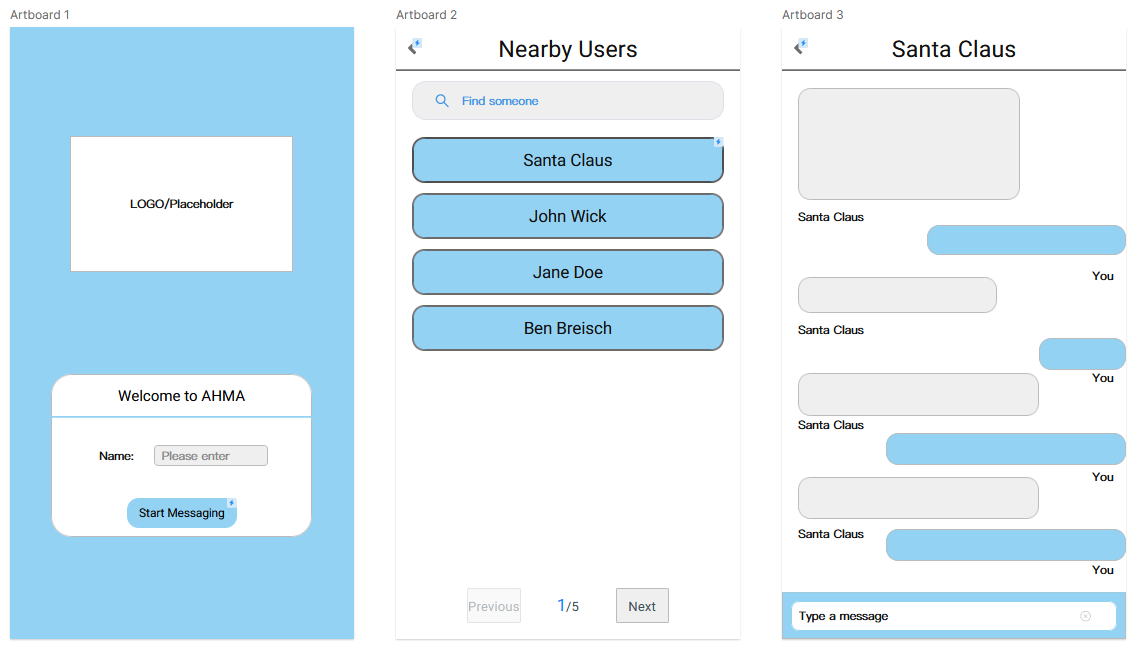
\includegraphics[scale=0.5]{wireframe.png} \\
\end{center}
Behind the scenes, this application will use a complex set of functions and internal storage structures. Devices may periodically broadcast beacon frames with routing information, tagged with usernames for each device. A possible technique could essentially be a fusion of AODV and DSDV routing. When the app is open on a device, it will listen for these beacon frames and update its routing table accordingly. If a device receives a frame destined for a different host, it will look up the host in its routing table and determine if it is reachable, forwarding the packet along if it is. When a frame is received at the destination host, it will detect errors with a checksum or CRC32 and reply with an ACK. Messages will likely be limited to 1024 characters in order to cut down on network latency and reduce packet loss. Conversations between users will be stored on the device.

\section{Evaluation Plan}
%      \item What experiments are you going to run?
\subsection{Scenarios}

We plan to do all of our evaluation and experimentation on live devices. One of our team members has an android device and we are currently investigating how to emulate more android devices or acquire dummy devices for experimentation. To gain a full picture of our application's performance we plan to test it in the following scenarios:

\begin{itemize}
    \item Single-hop communication
    \item Multi-hop communication
    \item New user event
    \item Dropping user event
    \item High pace usage
    \item File messages
    \item Low distance
    \item Maximum distance
\end{itemize}

The single-hop communication experiments will be performed with two devices which will have a single connection between them. The multi-hop communication experiments will use at least three devices and test the routing capabilities of the app. We will also test how quickly our solution can adapt to topology changes such as users opening the app or closing the app. That in particular is especially important since people are rarely just using a single app continuously. Typical users will flip quickly between several different apps while using their phone or device. Additionally, we will test the impact of high paced usage on network performance. Some users send messages back and forth as fast as their fingers can type and even do that with multiple different contacts. Most messaging apps also allow for users to send each other multimedia messages or files such as photos and videos. So that capability will be tested as well. Finally, it is always important to study how the physical environment will impact performance. So we will run these experiments at a close distance range and then push it as high as we can go. All of these scenarios will be combined into an array of experiments that we can use to fully capture the performance of our app.

%   \item What criteria and metrics are you going to use to evaluate your solutions?
\subsection{Metrics}

For each experiment we will record the following metrics:
\begin{itemize}
    \item Throughput
    \item Latency
    \item Packet loss rate
\end{itemize}
The throughput in this case is simply the data transmission rate throughout the whole network. So, all of the messages sent and received over time measured in data per second. The latency has multiple components that will each need to be analyzed individually as well as together. For example, there is latency from route acquisition, processing, potential queuing, transmission, propagation, re-transmission, etc. We will attempt to record as many of the individual components as possible. Finally, the packet loss rate is simply the rate at which a packet transmission fails and a re-transmission is required.

\subsection{Criteria}

There are two key results we are looking for by performing these experiments. The first is comparing our app to other existing solutions. We want to see if our approach of using WiFi-Direct performs better or worse than the approaches detailed in the related work section. Furthermore, we want to analyze specific areas and metrics so as to conclude the pros and cons of the different technologies. The second result is if our solution meets the user's needs. Does it have the necessary throughput, latency, and reliability to provide a good experience for the casual user? That result will tell us whether or not our solution is usable and functional for the problem.

The criteria for our first result is fairly straightforward. We will simply compare our recorded metrics directs against the best existing solution we can find. This will allow us to compare and contrast the different approaches directly. On the other hand, the criteria for our second result is much less straightforward. There is no benchmark for the minimum performance required on a messaging app. So we will evaluate the app against our own defined criteria of what is needed for a "good user experience".

These soft criteria are as follows:
\begin{itemize}
    \item Able to handle constant activity, fast paced messaging between multiple pairs of users.
    \item Scales to a large number of users, at least 10 in a small area.
    \item Low latency
          \begin{itemize}
              \item Less than one second for text messages
              \item Less then ten seconds for files, pictures, or videos
          \end{itemize}
    \item Reliable delivery, data gets delivered unless destination is unreachable.
\end{itemize}
These are the basic requirements for any messaging app to be useful. If any one of these are missing then the user experience is miserable.
A messaging app needs to keep up with even the fastest typer. We can put a character limit to restrict total message size, but that wouldn't stop a user from sending many large messages in quick succession. Therefore, it is important that the app can handle such usage. One speedy user shouldn't be able to cause themselves or other users to experience delay. We will need to find out how fast a person can send out messages at maximum and then use that as a throughput threshold for how fast our app needs to be.

Scalability is the next concern. If users can't send or receive messages in a crowded environment then the app is not very useful. Settings such as a school, apartment complex, or office may have many participating users trying to use the app at once. More participating devices in the network obviously increases the total network bandwidth, but does that increase in bandwidth outpace the increase in required throughput? We don't have the equipment required to test a truly large scale deployment of our app, but we can still analyze the impact of more participating devices. Then by weighing the increase in both bandwidth and throughput, we can estimate how well the application will scale.

Since our app sends messages locally to a destination, rather than traveling through a complex network of infrastructure nodes, users will expect it to be very quick. Therefore, low latency is also a requirement. Nobody likes to wait for something as simple as a message to send. Especially when some conversations are time sensitive. So the text messages themselves should send very quickly, with a small wait required for larger files.
Finally, messages need to be delivered. When a user sends a message they expect it to actually reach the destination. If that promise isn't upheld then that can cause confusion and frustration amongst users. If the destination is unreachable then the sending user needs to be alerted of this. This is a potential problem for our app as users could be hopping on and off the app at a rapid pace.

\section{Milestones} %(with dates)
The table below describes the milestones and associated due dates for each.
\begin{center}
    \begin{tabular}{ |c|c|c| }
        \hline
        Milestone                  & Explanation  \\ \hline
        Install Development Tools  & Oct 14, 2023 \\
        Initial Implementation     & Oct 21, 2023 \\
        Begin Final Report Writing & Nov 1, 2023  \\
        Finish App Implementation  & Nov 15,2023  \\
        Final Report Due           & Nov 22, 2023 \\
        \hline
    \end{tabular}
\end{center}


\bibliographystyle{acm}
\bibliography{refs}{}

\end{document}
